% Graphic for TeX using PGF
% Title: /home/marcel/Dokumente/1663_Datestrukturen/ea5_1_abb9.dia
% Creator: Dia v0.97.3
<<<<<<< HEAD
% CreationDate: Thu Jun  8 22:49:24 2017
=======
% CreationDate: Fri Jun  9 08:49:11 2017
>>>>>>> 69639f46859a02ebf2293365717ef7977f8a19fb
% For: marcel
% \usepackage{tikz}
% The following commands are not supported in PSTricks at present
% We define them conditionally, so when they are implemented,
% this pgf file will use them.
\ifx\du\undefined
  \newlength{\du}
\fi
\setlength{\du}{15\unitlength}
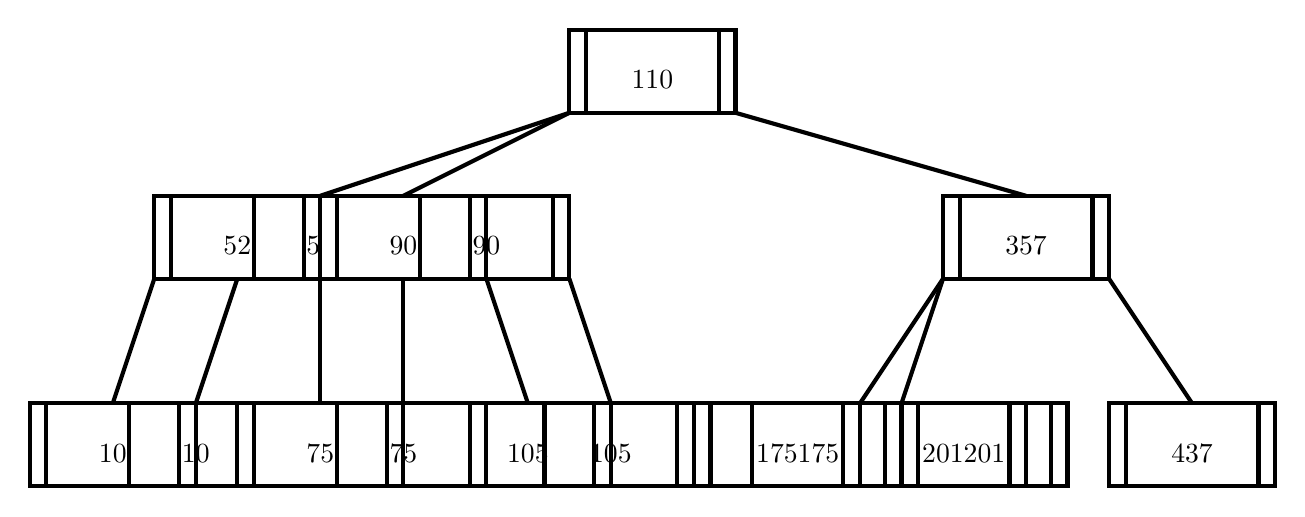
\begin{tikzpicture}
\pgftransformxscale{1.000000}
\pgftransformyscale{-1.000000}
\definecolor{dialinecolor}{rgb}{0.000000, 0.000000, 0.000000}
\pgfsetstrokecolor{dialinecolor}
\definecolor{dialinecolor}{rgb}{1.000000, 1.000000, 1.000000}
\pgfsetfillcolor{dialinecolor}
\pgfsetlinewidth{0.100000\du}
\pgfsetdash{}{0pt}
\pgfsetdash{}{0pt}
\pgfsetbuttcap
\pgfsetmiterjoin
\pgfsetlinewidth{0.100000\du}
\pgfsetbuttcap
\pgfsetmiterjoin
\pgfsetdash{}{0pt}
\definecolor{dialinecolor}{rgb}{1.000000, 1.000000, 1.000000}
\pgfsetfillcolor{dialinecolor}
<<<<<<< HEAD
\fill (16.000000\du,2.000000\du)--(16.000000\du,4.000000\du)--(20.000000\du,4.000000\du)--(20.000000\du,2.000000\du)--cycle;
\definecolor{dialinecolor}{rgb}{0.000000, 0.000000, 0.000000}
\pgfsetstrokecolor{dialinecolor}
\draw (16.000000\du,2.000000\du)--(16.000000\du,4.000000\du)--(20.000000\du,4.000000\du)--(20.000000\du,2.000000\du)--cycle;
=======
\fill (14.000000\du,2.000000\du)--(14.000000\du,4.000000\du)--(18.000000\du,4.000000\du)--(18.000000\du,2.000000\du)--cycle;
\definecolor{dialinecolor}{rgb}{0.000000, 0.000000, 0.000000}
\pgfsetstrokecolor{dialinecolor}
\draw (14.000000\du,2.000000\du)--(14.000000\du,4.000000\du)--(18.000000\du,4.000000\du)--(18.000000\du,2.000000\du)--cycle;
>>>>>>> 69639f46859a02ebf2293365717ef7977f8a19fb
\pgfsetbuttcap
\pgfsetmiterjoin
\pgfsetdash{}{0pt}
\definecolor{dialinecolor}{rgb}{0.000000, 0.000000, 0.000000}
\pgfsetstrokecolor{dialinecolor}
<<<<<<< HEAD
\draw (16.400000\du,2.000000\du)--(16.400000\du,4.000000\du);
=======
\draw (14.400000\du,2.000000\du)--(14.400000\du,4.000000\du);
>>>>>>> 69639f46859a02ebf2293365717ef7977f8a19fb
\pgfsetbuttcap
\pgfsetmiterjoin
\pgfsetdash{}{0pt}
\definecolor{dialinecolor}{rgb}{0.000000, 0.000000, 0.000000}
\pgfsetstrokecolor{dialinecolor}
<<<<<<< HEAD
\draw (19.600000\du,2.000000\du)--(19.600000\du,4.000000\du);
% setfont left to latex
\definecolor{dialinecolor}{rgb}{0.000000, 0.000000, 0.000000}
\pgfsetstrokecolor{dialinecolor}
\node at (18.000000\du,3.200000\du){52};
=======
\draw (17.600000\du,2.000000\du)--(17.600000\du,4.000000\du);
% setfont left to latex
\definecolor{dialinecolor}{rgb}{0.000000, 0.000000, 0.000000}
\pgfsetstrokecolor{dialinecolor}
\node at (16.000000\du,3.200000\du){52};
>>>>>>> 69639f46859a02ebf2293365717ef7977f8a19fb
\pgfsetlinewidth{0.100000\du}
\pgfsetdash{}{0pt}
\pgfsetdash{}{0pt}
\pgfsetbuttcap
\pgfsetmiterjoin
\pgfsetlinewidth{0.100000\du}
\pgfsetbuttcap
\pgfsetmiterjoin
\pgfsetdash{}{0pt}
\definecolor{dialinecolor}{rgb}{1.000000, 1.000000, 1.000000}
\pgfsetfillcolor{dialinecolor}
\fill (24.000000\du,-2.000000\du)--(24.000000\du,0.000000\du)--(28.000000\du,0.000000\du)--(28.000000\du,-2.000000\du)--cycle;
\definecolor{dialinecolor}{rgb}{0.000000, 0.000000, 0.000000}
\pgfsetstrokecolor{dialinecolor}
\draw (24.000000\du,-2.000000\du)--(24.000000\du,0.000000\du)--(28.000000\du,0.000000\du)--(28.000000\du,-2.000000\du)--cycle;
\pgfsetbuttcap
\pgfsetmiterjoin
\pgfsetdash{}{0pt}
\definecolor{dialinecolor}{rgb}{0.000000, 0.000000, 0.000000}
\pgfsetstrokecolor{dialinecolor}
\draw (24.400000\du,-2.000000\du)--(24.400000\du,0.000000\du);
\pgfsetbuttcap
\pgfsetmiterjoin
\pgfsetdash{}{0pt}
\definecolor{dialinecolor}{rgb}{0.000000, 0.000000, 0.000000}
\pgfsetstrokecolor{dialinecolor}
\draw (27.600000\du,-2.000000\du)--(27.600000\du,0.000000\du);
% setfont left to latex
\definecolor{dialinecolor}{rgb}{0.000000, 0.000000, 0.000000}
\pgfsetstrokecolor{dialinecolor}
\node at (26.000000\du,-0.800000\du){110};
\pgfsetlinewidth{0.100000\du}
\pgfsetdash{}{0pt}
\pgfsetdash{}{0pt}
\pgfsetbuttcap
\pgfsetmiterjoin
\pgfsetlinewidth{0.100000\du}
\pgfsetbuttcap
\pgfsetmiterjoin
\pgfsetdash{}{0pt}
\definecolor{dialinecolor}{rgb}{1.000000, 1.000000, 1.000000}
\pgfsetfillcolor{dialinecolor}
\fill (33.000000\du,2.000000\du)--(33.000000\du,4.000000\du)--(37.000000\du,4.000000\du)--(37.000000\du,2.000000\du)--cycle;
\definecolor{dialinecolor}{rgb}{0.000000, 0.000000, 0.000000}
\pgfsetstrokecolor{dialinecolor}
\draw (33.000000\du,2.000000\du)--(33.000000\du,4.000000\du)--(37.000000\du,4.000000\du)--(37.000000\du,2.000000\du)--cycle;
\pgfsetbuttcap
\pgfsetmiterjoin
\pgfsetdash{}{0pt}
\definecolor{dialinecolor}{rgb}{0.000000, 0.000000, 0.000000}
\pgfsetstrokecolor{dialinecolor}
\draw (33.400000\du,2.000000\du)--(33.400000\du,4.000000\du);
\pgfsetbuttcap
\pgfsetmiterjoin
\pgfsetdash{}{0pt}
\definecolor{dialinecolor}{rgb}{0.000000, 0.000000, 0.000000}
\pgfsetstrokecolor{dialinecolor}
\draw (36.600000\du,2.000000\du)--(36.600000\du,4.000000\du);
% setfont left to latex
\definecolor{dialinecolor}{rgb}{0.000000, 0.000000, 0.000000}
\pgfsetstrokecolor{dialinecolor}
\node at (35.000000\du,3.200000\du){357};
\pgfsetlinewidth{0.100000\du}
\pgfsetdash{}{0pt}
\pgfsetdash{}{0pt}
\pgfsetbuttcap
{
\definecolor{dialinecolor}{rgb}{0.000000, 0.000000, 0.000000}
\pgfsetfillcolor{dialinecolor}
% was here!!!
\definecolor{dialinecolor}{rgb}{0.000000, 0.000000, 0.000000}
\pgfsetstrokecolor{dialinecolor}
<<<<<<< HEAD
\draw (20.000000\du,4.000000\du)--(20.000000\du,6.951172\du);
=======
\draw (18.000000\du,4.000000\du)--(18.000000\du,6.951172\du);
>>>>>>> 69639f46859a02ebf2293365717ef7977f8a19fb
}
\pgfsetlinewidth{0.100000\du}
\pgfsetdash{}{0pt}
\pgfsetdash{}{0pt}
\pgfsetbuttcap
{
\definecolor{dialinecolor}{rgb}{0.000000, 0.000000, 0.000000}
\pgfsetfillcolor{dialinecolor}
% was here!!!
\definecolor{dialinecolor}{rgb}{0.000000, 0.000000, 0.000000}
\pgfsetstrokecolor{dialinecolor}
\draw (37.000000\du,4.000000\du)--(39.000000\du,7.000000\du);
}
\pgfsetlinewidth{0.100000\du}
\pgfsetdash{}{0pt}
\pgfsetdash{}{0pt}
\pgfsetbuttcap
\pgfsetmiterjoin
\pgfsetlinewidth{0.100000\du}
\pgfsetbuttcap
\pgfsetmiterjoin
\pgfsetdash{}{0pt}
\definecolor{dialinecolor}{rgb}{1.000000, 1.000000, 1.000000}
\pgfsetfillcolor{dialinecolor}
<<<<<<< HEAD
\fill (20.000000\du,2.000000\du)--(20.000000\du,4.000000\du)--(24.000000\du,4.000000\du)--(24.000000\du,2.000000\du)--cycle;
\definecolor{dialinecolor}{rgb}{0.000000, 0.000000, 0.000000}
\pgfsetstrokecolor{dialinecolor}
\draw (20.000000\du,2.000000\du)--(20.000000\du,4.000000\du)--(24.000000\du,4.000000\du)--(24.000000\du,2.000000\du)--cycle;
=======
\fill (18.000000\du,2.000000\du)--(18.000000\du,4.000000\du)--(22.000000\du,4.000000\du)--(22.000000\du,2.000000\du)--cycle;
\definecolor{dialinecolor}{rgb}{0.000000, 0.000000, 0.000000}
\pgfsetstrokecolor{dialinecolor}
\draw (18.000000\du,2.000000\du)--(18.000000\du,4.000000\du)--(22.000000\du,4.000000\du)--(22.000000\du,2.000000\du)--cycle;
>>>>>>> 69639f46859a02ebf2293365717ef7977f8a19fb
\pgfsetbuttcap
\pgfsetmiterjoin
\pgfsetdash{}{0pt}
\definecolor{dialinecolor}{rgb}{0.000000, 0.000000, 0.000000}
\pgfsetstrokecolor{dialinecolor}
<<<<<<< HEAD
\draw (20.400000\du,2.000000\du)--(20.400000\du,4.000000\du);
=======
\draw (18.400000\du,2.000000\du)--(18.400000\du,4.000000\du);
>>>>>>> 69639f46859a02ebf2293365717ef7977f8a19fb
\pgfsetbuttcap
\pgfsetmiterjoin
\pgfsetdash{}{0pt}
\definecolor{dialinecolor}{rgb}{0.000000, 0.000000, 0.000000}
\pgfsetstrokecolor{dialinecolor}
<<<<<<< HEAD
\draw (23.600000\du,2.000000\du)--(23.600000\du,4.000000\du);
% setfont left to latex
\definecolor{dialinecolor}{rgb}{0.000000, 0.000000, 0.000000}
\pgfsetstrokecolor{dialinecolor}
\node at (22.000000\du,3.200000\du){90};
=======
\draw (21.600000\du,2.000000\du)--(21.600000\du,4.000000\du);
% setfont left to latex
\definecolor{dialinecolor}{rgb}{0.000000, 0.000000, 0.000000}
\pgfsetstrokecolor{dialinecolor}
\node at (20.000000\du,3.200000\du){90};
>>>>>>> 69639f46859a02ebf2293365717ef7977f8a19fb
\pgfsetlinewidth{0.100000\du}
\pgfsetdash{}{0pt}
\pgfsetdash{}{0pt}
\pgfsetbuttcap
\pgfsetmiterjoin
\pgfsetlinewidth{0.100000\du}
\pgfsetbuttcap
\pgfsetmiterjoin
\pgfsetdash{}{0pt}
\definecolor{dialinecolor}{rgb}{1.000000, 1.000000, 1.000000}
\pgfsetfillcolor{dialinecolor}
<<<<<<< HEAD
\fill (32.000000\du,7.000000\du)--(32.000000\du,9.000000\du)--(36.000000\du,9.000000\du)--(36.000000\du,7.000000\du)--cycle;
\definecolor{dialinecolor}{rgb}{0.000000, 0.000000, 0.000000}
\pgfsetstrokecolor{dialinecolor}
\draw (32.000000\du,7.000000\du)--(32.000000\du,9.000000\du)--(36.000000\du,9.000000\du)--(36.000000\du,7.000000\du)--cycle;
=======
\fill (31.000000\du,7.000000\du)--(31.000000\du,9.000000\du)--(35.000000\du,9.000000\du)--(35.000000\du,7.000000\du)--cycle;
\definecolor{dialinecolor}{rgb}{0.000000, 0.000000, 0.000000}
\pgfsetstrokecolor{dialinecolor}
\draw (31.000000\du,7.000000\du)--(31.000000\du,9.000000\du)--(35.000000\du,9.000000\du)--(35.000000\du,7.000000\du)--cycle;
>>>>>>> 69639f46859a02ebf2293365717ef7977f8a19fb
\pgfsetbuttcap
\pgfsetmiterjoin
\pgfsetdash{}{0pt}
\definecolor{dialinecolor}{rgb}{0.000000, 0.000000, 0.000000}
\pgfsetstrokecolor{dialinecolor}
<<<<<<< HEAD
\draw (32.400000\du,7.000000\du)--(32.400000\du,9.000000\du);
=======
\draw (31.400000\du,7.000000\du)--(31.400000\du,9.000000\du);
>>>>>>> 69639f46859a02ebf2293365717ef7977f8a19fb
\pgfsetbuttcap
\pgfsetmiterjoin
\pgfsetdash{}{0pt}
\definecolor{dialinecolor}{rgb}{0.000000, 0.000000, 0.000000}
\pgfsetstrokecolor{dialinecolor}
<<<<<<< HEAD
\draw (35.600000\du,7.000000\du)--(35.600000\du,9.000000\du);
% setfont left to latex
\definecolor{dialinecolor}{rgb}{0.000000, 0.000000, 0.000000}
\pgfsetstrokecolor{dialinecolor}
\node at (34.000000\du,8.200000\du){201};
=======
\draw (34.600000\du,7.000000\du)--(34.600000\du,9.000000\du);
% setfont left to latex
\definecolor{dialinecolor}{rgb}{0.000000, 0.000000, 0.000000}
\pgfsetstrokecolor{dialinecolor}
\node at (33.000000\du,8.200000\du){201};
>>>>>>> 69639f46859a02ebf2293365717ef7977f8a19fb
\pgfsetlinewidth{0.100000\du}
\pgfsetdash{}{0pt}
\pgfsetdash{}{0pt}
\pgfsetbuttcap
\pgfsetmiterjoin
\pgfsetlinewidth{0.100000\du}
\pgfsetbuttcap
\pgfsetmiterjoin
\pgfsetdash{}{0pt}
\definecolor{dialinecolor}{rgb}{1.000000, 1.000000, 1.000000}
\pgfsetfillcolor{dialinecolor}
\fill (37.000000\du,7.000000\du)--(37.000000\du,9.000000\du)--(41.000000\du,9.000000\du)--(41.000000\du,7.000000\du)--cycle;
\definecolor{dialinecolor}{rgb}{0.000000, 0.000000, 0.000000}
\pgfsetstrokecolor{dialinecolor}
\draw (37.000000\du,7.000000\du)--(37.000000\du,9.000000\du)--(41.000000\du,9.000000\du)--(41.000000\du,7.000000\du)--cycle;
\pgfsetbuttcap
\pgfsetmiterjoin
\pgfsetdash{}{0pt}
\definecolor{dialinecolor}{rgb}{0.000000, 0.000000, 0.000000}
\pgfsetstrokecolor{dialinecolor}
\draw (37.400000\du,7.000000\du)--(37.400000\du,9.000000\du);
\pgfsetbuttcap
\pgfsetmiterjoin
\pgfsetdash{}{0pt}
\definecolor{dialinecolor}{rgb}{0.000000, 0.000000, 0.000000}
\pgfsetstrokecolor{dialinecolor}
\draw (40.600000\du,7.000000\du)--(40.600000\du,9.000000\du);
% setfont left to latex
\definecolor{dialinecolor}{rgb}{0.000000, 0.000000, 0.000000}
\pgfsetstrokecolor{dialinecolor}
\node at (39.000000\du,8.200000\du){437};
\pgfsetlinewidth{0.100000\du}
\pgfsetdash{}{0pt}
\pgfsetdash{}{0pt}
\pgfsetbuttcap
{
\definecolor{dialinecolor}{rgb}{0.000000, 0.000000, 0.000000}
\pgfsetfillcolor{dialinecolor}
% was here!!!
\definecolor{dialinecolor}{rgb}{0.000000, 0.000000, 0.000000}
\pgfsetstrokecolor{dialinecolor}
<<<<<<< HEAD
\draw (33.000000\du,4.000000\du)--(32.000000\du,7.000000\du);
=======
\draw (33.000000\du,4.000000\du)--(31.000000\du,7.000000\du);
>>>>>>> 69639f46859a02ebf2293365717ef7977f8a19fb
}
\pgfsetlinewidth{0.100000\du}
\pgfsetdash{}{0pt}
\pgfsetdash{}{0pt}
\pgfsetbuttcap
\pgfsetmiterjoin
\pgfsetlinewidth{0.100000\du}
\pgfsetbuttcap
\pgfsetmiterjoin
\pgfsetdash{}{0pt}
\definecolor{dialinecolor}{rgb}{1.000000, 1.000000, 1.000000}
\pgfsetfillcolor{dialinecolor}
<<<<<<< HEAD
\fill (13.000000\du,7.000000\du)--(13.000000\du,9.000000\du)--(17.000000\du,9.000000\du)--(17.000000\du,7.000000\du)--cycle;
\definecolor{dialinecolor}{rgb}{0.000000, 0.000000, 0.000000}
\pgfsetstrokecolor{dialinecolor}
\draw (13.000000\du,7.000000\du)--(13.000000\du,9.000000\du)--(17.000000\du,9.000000\du)--(17.000000\du,7.000000\du)--cycle;
=======
\fill (11.000000\du,7.000000\du)--(11.000000\du,9.000000\du)--(15.000000\du,9.000000\du)--(15.000000\du,7.000000\du)--cycle;
\definecolor{dialinecolor}{rgb}{0.000000, 0.000000, 0.000000}
\pgfsetstrokecolor{dialinecolor}
\draw (11.000000\du,7.000000\du)--(11.000000\du,9.000000\du)--(15.000000\du,9.000000\du)--(15.000000\du,7.000000\du)--cycle;
>>>>>>> 69639f46859a02ebf2293365717ef7977f8a19fb
\pgfsetbuttcap
\pgfsetmiterjoin
\pgfsetdash{}{0pt}
\definecolor{dialinecolor}{rgb}{0.000000, 0.000000, 0.000000}
\pgfsetstrokecolor{dialinecolor}
<<<<<<< HEAD
\draw (13.400000\du,7.000000\du)--(13.400000\du,9.000000\du);
=======
\draw (11.400000\du,7.000000\du)--(11.400000\du,9.000000\du);
>>>>>>> 69639f46859a02ebf2293365717ef7977f8a19fb
\pgfsetbuttcap
\pgfsetmiterjoin
\pgfsetdash{}{0pt}
\definecolor{dialinecolor}{rgb}{0.000000, 0.000000, 0.000000}
\pgfsetstrokecolor{dialinecolor}
<<<<<<< HEAD
\draw (16.600000\du,7.000000\du)--(16.600000\du,9.000000\du);
% setfont left to latex
\definecolor{dialinecolor}{rgb}{0.000000, 0.000000, 0.000000}
\pgfsetstrokecolor{dialinecolor}
\node at (15.000000\du,8.200000\du){10};
=======
\draw (14.600000\du,7.000000\du)--(14.600000\du,9.000000\du);
% setfont left to latex
\definecolor{dialinecolor}{rgb}{0.000000, 0.000000, 0.000000}
\pgfsetstrokecolor{dialinecolor}
\node at (13.000000\du,8.200000\du){10};
>>>>>>> 69639f46859a02ebf2293365717ef7977f8a19fb
\pgfsetlinewidth{0.100000\du}
\pgfsetdash{}{0pt}
\pgfsetdash{}{0pt}
\pgfsetbuttcap
{
\definecolor{dialinecolor}{rgb}{0.000000, 0.000000, 0.000000}
\pgfsetfillcolor{dialinecolor}
% was here!!!
\definecolor{dialinecolor}{rgb}{0.000000, 0.000000, 0.000000}
\pgfsetstrokecolor{dialinecolor}
<<<<<<< HEAD
\draw (16.000000\du,4.000000\du)--(15.000000\du,7.000000\du);
=======
\draw (14.000000\du,4.000000\du)--(13.000000\du,7.000000\du);
>>>>>>> 69639f46859a02ebf2293365717ef7977f8a19fb
}
\pgfsetlinewidth{0.100000\du}
\pgfsetdash{}{0pt}
\pgfsetdash{}{0pt}
\pgfsetbuttcap
{
\definecolor{dialinecolor}{rgb}{0.000000, 0.000000, 0.000000}
\pgfsetfillcolor{dialinecolor}
% was here!!!
\definecolor{dialinecolor}{rgb}{0.000000, 0.000000, 0.000000}
\pgfsetstrokecolor{dialinecolor}
<<<<<<< HEAD
\draw (24.000000\du,0.000000\du)--(20.000000\du,2.000000\du);
=======
\draw (24.000000\du,0.000000\du)--(18.000000\du,2.000000\du);
>>>>>>> 69639f46859a02ebf2293365717ef7977f8a19fb
}
\pgfsetlinewidth{0.100000\du}
\pgfsetdash{}{0pt}
\pgfsetdash{}{0pt}
\pgfsetbuttcap
{
\definecolor{dialinecolor}{rgb}{0.000000, 0.000000, 0.000000}
\pgfsetfillcolor{dialinecolor}
% was here!!!
\definecolor{dialinecolor}{rgb}{0.000000, 0.000000, 0.000000}
\pgfsetstrokecolor{dialinecolor}
\draw (28.000000\du,0.000000\du)--(35.000000\du,2.000000\du);
}
\pgfsetlinewidth{0.100000\du}
\pgfsetdash{}{0pt}
\pgfsetdash{}{0pt}
\pgfsetbuttcap
\pgfsetmiterjoin
\pgfsetlinewidth{0.100000\du}
\pgfsetbuttcap
\pgfsetmiterjoin
\pgfsetdash{}{0pt}
\definecolor{dialinecolor}{rgb}{1.000000, 1.000000, 1.000000}
\pgfsetfillcolor{dialinecolor}
<<<<<<< HEAD
\fill (23.000000\du,7.000000\du)--(23.000000\du,9.000000\du)--(27.000000\du,9.000000\du)--(27.000000\du,7.000000\du)--cycle;
\definecolor{dialinecolor}{rgb}{0.000000, 0.000000, 0.000000}
\pgfsetstrokecolor{dialinecolor}
\draw (23.000000\du,7.000000\du)--(23.000000\du,9.000000\du)--(27.000000\du,9.000000\du)--(27.000000\du,7.000000\du)--cycle;
=======
\fill (21.000000\du,7.000000\du)--(21.000000\du,9.000000\du)--(25.000000\du,9.000000\du)--(25.000000\du,7.000000\du)--cycle;
\definecolor{dialinecolor}{rgb}{0.000000, 0.000000, 0.000000}
\pgfsetstrokecolor{dialinecolor}
\draw (21.000000\du,7.000000\du)--(21.000000\du,9.000000\du)--(25.000000\du,9.000000\du)--(25.000000\du,7.000000\du)--cycle;
>>>>>>> 69639f46859a02ebf2293365717ef7977f8a19fb
\pgfsetbuttcap
\pgfsetmiterjoin
\pgfsetdash{}{0pt}
\definecolor{dialinecolor}{rgb}{0.000000, 0.000000, 0.000000}
\pgfsetstrokecolor{dialinecolor}
<<<<<<< HEAD
\draw (23.400000\du,7.000000\du)--(23.400000\du,9.000000\du);
=======
\draw (21.400000\du,7.000000\du)--(21.400000\du,9.000000\du);
>>>>>>> 69639f46859a02ebf2293365717ef7977f8a19fb
\pgfsetbuttcap
\pgfsetmiterjoin
\pgfsetdash{}{0pt}
\definecolor{dialinecolor}{rgb}{0.000000, 0.000000, 0.000000}
\pgfsetstrokecolor{dialinecolor}
<<<<<<< HEAD
\draw (26.600000\du,7.000000\du)--(26.600000\du,9.000000\du);
% setfont left to latex
\definecolor{dialinecolor}{rgb}{0.000000, 0.000000, 0.000000}
\pgfsetstrokecolor{dialinecolor}
\node at (25.000000\du,8.200000\du){105};
=======
\draw (24.600000\du,7.000000\du)--(24.600000\du,9.000000\du);
% setfont left to latex
\definecolor{dialinecolor}{rgb}{0.000000, 0.000000, 0.000000}
\pgfsetstrokecolor{dialinecolor}
\node at (23.000000\du,8.200000\du){105};
>>>>>>> 69639f46859a02ebf2293365717ef7977f8a19fb
\pgfsetlinewidth{0.100000\du}
\pgfsetdash{}{0pt}
\pgfsetdash{}{0pt}
\pgfsetbuttcap
\pgfsetmiterjoin
\pgfsetlinewidth{0.100000\du}
\pgfsetbuttcap
\pgfsetmiterjoin
\pgfsetdash{}{0pt}
\definecolor{dialinecolor}{rgb}{1.000000, 1.000000, 1.000000}
\pgfsetfillcolor{dialinecolor}
<<<<<<< HEAD
\fill (28.000000\du,7.000000\du)--(28.000000\du,9.000000\du)--(32.000000\du,9.000000\du)--(32.000000\du,7.000000\du)--cycle;
\definecolor{dialinecolor}{rgb}{0.000000, 0.000000, 0.000000}
\pgfsetstrokecolor{dialinecolor}
\draw (28.000000\du,7.000000\du)--(28.000000\du,9.000000\du)--(32.000000\du,9.000000\du)--(32.000000\du,7.000000\du)--cycle;
=======
\fill (27.000000\du,7.000000\du)--(27.000000\du,9.000000\du)--(31.000000\du,9.000000\du)--(31.000000\du,7.000000\du)--cycle;
\definecolor{dialinecolor}{rgb}{0.000000, 0.000000, 0.000000}
\pgfsetstrokecolor{dialinecolor}
\draw (27.000000\du,7.000000\du)--(27.000000\du,9.000000\du)--(31.000000\du,9.000000\du)--(31.000000\du,7.000000\du)--cycle;
>>>>>>> 69639f46859a02ebf2293365717ef7977f8a19fb
\pgfsetbuttcap
\pgfsetmiterjoin
\pgfsetdash{}{0pt}
\definecolor{dialinecolor}{rgb}{0.000000, 0.000000, 0.000000}
\pgfsetstrokecolor{dialinecolor}
<<<<<<< HEAD
\draw (28.400000\du,7.000000\du)--(28.400000\du,9.000000\du);
=======
\draw (27.400000\du,7.000000\du)--(27.400000\du,9.000000\du);
>>>>>>> 69639f46859a02ebf2293365717ef7977f8a19fb
\pgfsetbuttcap
\pgfsetmiterjoin
\pgfsetdash{}{0pt}
\definecolor{dialinecolor}{rgb}{0.000000, 0.000000, 0.000000}
\pgfsetstrokecolor{dialinecolor}
<<<<<<< HEAD
\draw (31.600000\du,7.000000\du)--(31.600000\du,9.000000\du);
% setfont left to latex
\definecolor{dialinecolor}{rgb}{0.000000, 0.000000, 0.000000}
\pgfsetstrokecolor{dialinecolor}
\node at (30.000000\du,8.200000\du){175};
=======
\draw (30.600000\du,7.000000\du)--(30.600000\du,9.000000\du);
% setfont left to latex
\definecolor{dialinecolor}{rgb}{0.000000, 0.000000, 0.000000}
\pgfsetstrokecolor{dialinecolor}
\node at (29.000000\du,8.200000\du){175};
>>>>>>> 69639f46859a02ebf2293365717ef7977f8a19fb
\pgfsetlinewidth{0.100000\du}
\pgfsetdash{}{0pt}
\pgfsetdash{}{0pt}
\pgfsetbuttcap
\pgfsetmiterjoin
\pgfsetlinewidth{0.100000\du}
\pgfsetbuttcap
\pgfsetmiterjoin
\pgfsetdash{}{0pt}
\definecolor{dialinecolor}{rgb}{1.000000, 1.000000, 1.000000}
\pgfsetfillcolor{dialinecolor}
<<<<<<< HEAD
\fill (18.000000\du,7.000000\du)--(18.000000\du,9.000000\du)--(22.000000\du,9.000000\du)--(22.000000\du,7.000000\du)--cycle;
\definecolor{dialinecolor}{rgb}{0.000000, 0.000000, 0.000000}
\pgfsetstrokecolor{dialinecolor}
\draw (18.000000\du,7.000000\du)--(18.000000\du,9.000000\du)--(22.000000\du,9.000000\du)--(22.000000\du,7.000000\du)--cycle;
=======
\fill (16.000000\du,7.000000\du)--(16.000000\du,9.000000\du)--(20.000000\du,9.000000\du)--(20.000000\du,7.000000\du)--cycle;
\definecolor{dialinecolor}{rgb}{0.000000, 0.000000, 0.000000}
\pgfsetstrokecolor{dialinecolor}
\draw (16.000000\du,7.000000\du)--(16.000000\du,9.000000\du)--(20.000000\du,9.000000\du)--(20.000000\du,7.000000\du)--cycle;
>>>>>>> 69639f46859a02ebf2293365717ef7977f8a19fb
\pgfsetbuttcap
\pgfsetmiterjoin
\pgfsetdash{}{0pt}
\definecolor{dialinecolor}{rgb}{0.000000, 0.000000, 0.000000}
\pgfsetstrokecolor{dialinecolor}
<<<<<<< HEAD
\draw (18.400000\du,7.000000\du)--(18.400000\du,9.000000\du);
=======
\draw (16.400000\du,7.000000\du)--(16.400000\du,9.000000\du);
>>>>>>> 69639f46859a02ebf2293365717ef7977f8a19fb
\pgfsetbuttcap
\pgfsetmiterjoin
\pgfsetdash{}{0pt}
\definecolor{dialinecolor}{rgb}{0.000000, 0.000000, 0.000000}
\pgfsetstrokecolor{dialinecolor}
<<<<<<< HEAD
\draw (21.600000\du,7.000000\du)--(21.600000\du,9.000000\du);
% setfont left to latex
\definecolor{dialinecolor}{rgb}{0.000000, 0.000000, 0.000000}
\pgfsetstrokecolor{dialinecolor}
\node at (20.000000\du,8.200000\du){75};
=======
\draw (19.600000\du,7.000000\du)--(19.600000\du,9.000000\du);
% setfont left to latex
\definecolor{dialinecolor}{rgb}{0.000000, 0.000000, 0.000000}
\pgfsetstrokecolor{dialinecolor}
\node at (18.000000\du,8.200000\du){75};
>>>>>>> 69639f46859a02ebf2293365717ef7977f8a19fb
\pgfsetlinewidth{0.100000\du}
\pgfsetdash{}{0pt}
\pgfsetdash{}{0pt}
\pgfsetbuttcap
{
\definecolor{dialinecolor}{rgb}{0.000000, 0.000000, 0.000000}
\pgfsetfillcolor{dialinecolor}
% was here!!!
\definecolor{dialinecolor}{rgb}{0.000000, 0.000000, 0.000000}
\pgfsetstrokecolor{dialinecolor}
<<<<<<< HEAD
\draw (24.000000\du,4.000000\du)--(25.000000\du,7.000000\du);
=======
\draw (22.000000\du,4.000000\du)--(23.000000\du,7.000000\du);
>>>>>>> 69639f46859a02ebf2293365717ef7977f8a19fb
}
\end{tikzpicture}
